\section{Перетворення Фур'є}
Перетворення Фур’є дає можливість подати складний сигнал у вигляді суми більш простих сигналів, зокрема у вигляді найпростіших гармонічних коливань. Перетворення Фур’є ми здійснювали на осцилографі за допомогою меню \textbf{MATH}, режиму \textbf{FFT} (швидке перетворення Фур'є – режим, що дозволяє знайти частотні компоненти (спектр) сигналу), за такою послідовністю дій:

\begin{enumerate}
    \item \textbf{АВТОУСТ}.
    \item \textbf{ВЕРТИК. ПОЛОЖЕНИЕ} та \textbf{ГОРИЗОНТ. ПОЛОЖЕНИЕ} (вирівнювали сигнал по центру екрана).
    \item \textbf{ВОЛЬТ/ДЕЛ} (поки не відображався весь сигнал).
    \item \textbf{MATH} та \textbf{FFT}.
    \item обирали канал, сигнал якого перетворювали.
\end{enumerate}

В результаті ми отримали такі перетворення Фур'є: \\
\\
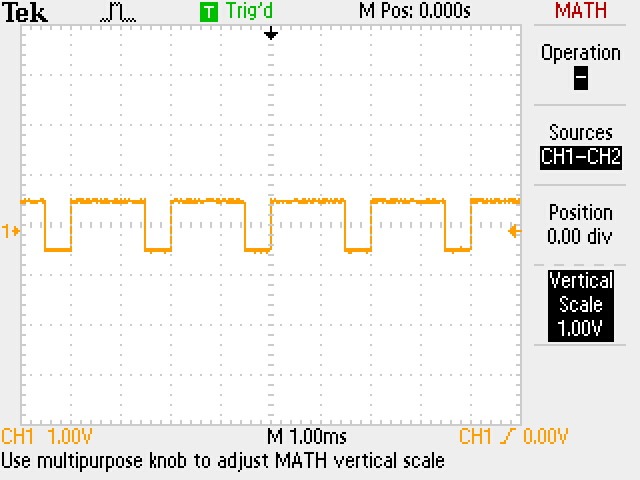
\includegraphics[width=\textwidth/2]{1-lab/res/1a.JPG}
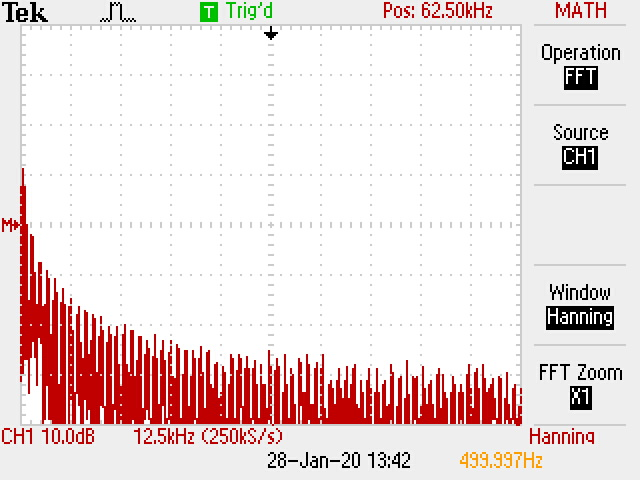
\includegraphics[width=\textwidth/2]{1-lab/res/1b.JPG} \\
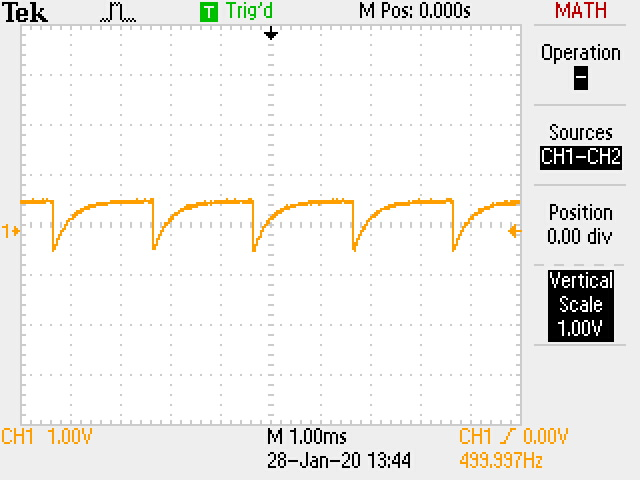
\includegraphics[width=\textwidth/2]{1-lab/res/2a.JPG}
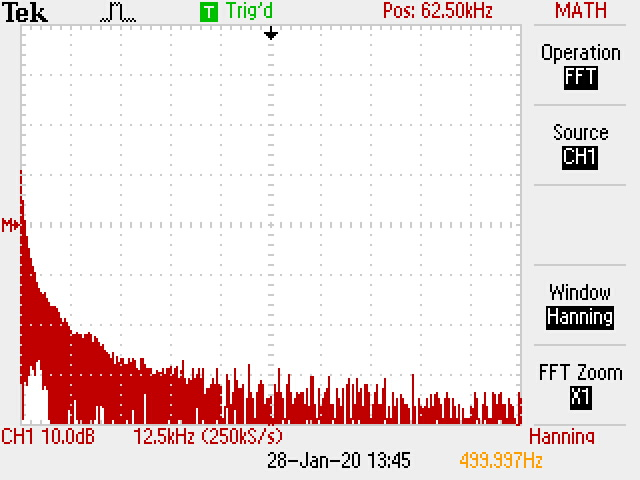
\includegraphics[width=\textwidth/2]{1-lab/res/2b.JPG}
